\subsection{Avalanche : ajout d'un DAG}%\tronly{}{\vspace{-0.5em}}

%O Avalanche consists of multiple single-decree Snowball instances instantiated as a multi-decree protocol that
%O maintains a dynamic, append-only directed acyclic graph (DAG) of all known transactions.
Avalanche consiste en plusieurs instance Snowball à décret unique instanciées en tant que protocole multi-décrets qui maintient un graphe orienté acyclique (\emph{Directed Acyclic Graph},  DAG) dynamique en ajout seul de toutes les transactions connues.
%O The DAG has a single sink that is the \emph{genesis vertex}.
Le DAG a un nœud terminal (\emph{sink}) unique qui est le \emph{genesis vertex}, le sommet genèse. % HOULA sink ? 
%O Maintaining a DAG provides two significant benefits.
L'emploi d'un DAG procure deux avantages :
%O First, it improves efficiency, because a single vote on a DAG vertex implicitly votes for all tran
%O sactions on the path to the genesis vertex.
D'abord, il est plus efficient car un vote sur un sommet vote implicitement pour toutes les transactions sur le chemin vers le sommet genèse.
%O Second, it also improves security, because the DAG intertwines the fate of transactions, similar to the Bitcoin blockchain.
Ensuite, il améliore également la sécurité parce que le entrelace le sort des transactions, similaire en cela à la blockchain de Bitcoin.
%O This renders past decisions difficult to undo without the approval of correct nodes.
Cela rend les décisions passées difficiles à défaire sans l'approbation des nœuds corrects.


% Avalanche's DAG embodies all the transactions that have been proposed to the system, where each transaction is represented as a vertex.
% The DAG is rooted at a protocol-defined, well-known \emph{genesis} vertex.
%O When a client creates a transaction, it names one or more \emph{parents}, which are included inseparably in the transaction and form the edges of the DAG\@.
Quand un client crée une transaction, il nomme un ou plusieurs \emph{parents}, et ceux-ci sont inclus de façon inséparable dans la transaction et forment les bords du DAG\@.
%O The parent-child relationships encoded in the DAG may, but do not need to, correspond to application-specific dependencies; for instance, a child transaction need not spend or have any relationship with the funds received in the parent transaction.
Les relations parent-enfant codées dans le DAG peuvent, sans obligation, correspondre à des dépendances spécifiques aux applications ; par exemple, la transaction d'un enfant ne dépense pas nécessairement, ni n'a forcément de relation avec les fonds reçus lors de la transaction parent.
% These additional relationships entangle the fate of previous decisions made by the system.
%O We use the term \emph{ancestor set} to refer to all transactions reachable via parent edges back in history, and \emph{progeny} to refer to all children transactions and their offspring.
Nous utilisons le terme \emph{ensemble ancêtre} pour nous référer à toutes les transactions accessibles par les arêtes parent historisées, et \emph{progéniture} pour nous référer à toutes les transactions enfant et leur descendance.

%O The central challenge in the maintenance of the DAG is to choose among \emph{conflicting transactions}.
Le principal défi de la maintenance du DAG est de choisir parmi des \emph{trasactions conflictuelles}.
%O The notion of conflict is application-defined and transitive, forming an equivalence relation.
La notion de conflit est définie par l'application et est transitive, formant une relation d'équivalence.
%O In our cryptocurrency application, transactions that spend the same funds (\emph{double-spends}) conflict, and form a \emph{conflict set}
Dans notre application de cryptomonnaie, les transactions qui dépensent les mêmes fonds (\emph{double-dépense}) entrent en conflit et forment un \emph{ensemble de conflit}
%(Figure~\tronly{\ref{fig:dag-conflict-set}}{\ref{fig:dag-cd}})
%O (shaded regions in Figure~\ref{fig:dag-cd}), out of which only a single one can be accepted.
(régions ombrées en Figure~\ref{fig:dag-cd}), duquel une seule peut être acceptée.
%O Note that the conflict set of a virtuous transaction is always a singleton.
On note que l'ensemble de conflit d'une transaction vertueuse est toujours un singleton.
%Note that the graph structure of transactions that spend depend on each other, also known as the UTXO graph, is completely independent of the DAG that Avalanche maintains. As a result, any two vertices may be in conflict. Figure~\ref{fig:dag-conflicting-set} shows an example.
 
%\tronly{
%\begin{figure}\begin{center}
%    \definecolor{lightgray}{HTML}{dddddd}
\definecolor{medgray}{HTML}{cccccc}
\definecolor{medgray2}{HTML}{bbbbbb}
\definecolor{darkgray}{HTML}{aaaaaa}
\definecolor{lightgp}{HTML}{ddddee}
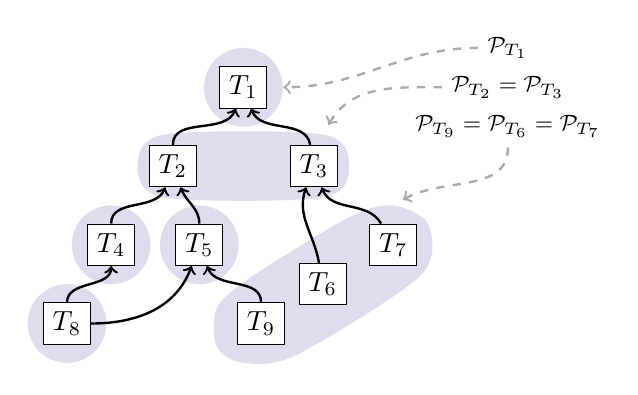
\begin{tikzpicture}[x=1.12cm]
    \begin{scope}[all/.style={draw,fill=white,minimum height=0.5cm, minimum width=0.5cm},line width=0.08ex]
        \node[fill=lightgp, circle,minimum width=1cm] (pt1) at (0, 0) {};
        \node[fill=lightgp, circle,minimum width=1cm] (pt4) at (-1.5, -2) {};
        \node[fill=lightgp, circle,minimum width=1cm] (pt5) at (-0.5, -2) {};
        \node[fill=lightgp, circle,minimum width=1cm] (pt6) at (-2, -3) {};
        \fill[color=lightgp] plot[smooth cycle] coordinates { (1.2, -1) (0.9, -1.4) (-0.9, -1.4) (-1.2, -1) (-0.9, -0.6) (0.9, -0.6)} node (pt2) {};
        \fill[color=lightgp] plot[smooth cycle] coordinates {(2.1, -1.75) (2, -2.4) (0.6, -3.4) (0, -3.5) (-0.3, -3.3)(-0.3, -2.8) (0.1, -2.4) (1.2, -1.65) (1.7, -1.5) } node (pt3) {};
        \node[all, draw] (b0) at (0, 0) {$T_1$};
        \node[all, draw] (b1) at (-0.8, -1) {$T_2$};
        \node[all, draw] (b2) at (0.8, -1) {$T_3$};
        \node[all, draw] (b3) at (-1.5, -2) {$T_4$};
        \node[all, draw] (b4) at (-0.5, -2) {$T_5$};
        \node[all, draw] (b5) at (0.9, -2.5) {$T_6$};
        \node[all, draw] (b6) at (1.7, -2) {$T_7$};
        \node[all, draw] (b7) at (-2, -3) {$T_8$};
        \node[all, draw] (b8) at (0.2, -3) {$T_9$};
        \begin{scope}[line width=0.2ex]
        \path[->] (b1) edge[out=90, in=-110] node[sloped,above] {} (b0) ;
        \path[->] (b2) edge[out=100, in=-70] node[sloped,above] {} (b0) ;
        \path[->] (b3) edge[out=90, in=-110] node[sloped,above] {} (b1) ;
        \path[->] (b4) edge[out=90, in=-70] node[sloped,above] {} (b1) ;
        \path[->] (b5) edge[out=100, in=-110] node[sloped,above] {} (b2) ;
        \path[->] (b6) edge[out=120, in=-70] node[sloped,above] {} (b2) ;
        \path[->] (b7) edge[out=90, in=-90] node[sloped,above] {} (b3) ;
        \path[->] (b7) edge[out=0, in=-110] node[sloped,above] {} (b4) ;
        \path[->] (b8) edge[out=90, in=-70] node[sloped,above] {} (b4) ;
        \end{scope}
        \node[] (p1) at (3, 0.5) {\footnotesize$\mathcal{P}_{T_1}$};
        \node[] (p2) at (3, 0) {\footnotesize$\mathcal{P}_{T_2} = \mathcal{P}_{T_3}$};
        \node[] (p3) at (3, -0.5) {\footnotesize$\mathcal{P}_{T_9} = \mathcal{P}_{T_6} = \mathcal{P}_{T_7}$};
        \begin{scope}[color=darkgray,dashed,line width=0.2ex]
        \path[->] (p1) edge[out=180, in=0] node[sloped,above] {} (pt1) ;
        \path[->] (p2) edge[out=180, in=60] node[sloped,above] {} (pt2) ;
        \path[->] (p3) edge[out=-90, in=30] node[sloped,above] {} (pt3) ;
        \end{scope}
    \end{scope}
\end{tikzpicture}

%    \captionof{figure}{DAG vertices partitioned by conflict sets. At most one vertex in each shaded region will be accepted.}\label{fig:dag-conflict-set}
%\end{center}
%\end{figure}
%}{}

%O Avalanche instantiates a Snowball instance for each conflict set.
Avalanche instancie une instance de Snowball pour chaque ensemble de conflit.
%O Whereas Snowball uses repeated queries and multiple counters to capture the amount of confidence built in conflicting transactions (colors),
%O Avalanche takes advantage of the DAG structure and uses a transaction's progeny.
Alors que Snowball utilise des requêtes répétées et plusieurs compteurs pour capturer le degré de confiance associé aux transactions conflictuelles (couleurs),
Avalanche profite de la structure du DAG et utilise la progéniture d'une transaction.
%O Specifically, when a transaction $T$ is queried, all transactions reachable from $T$ by following the DAG edges are implicitly part of the query.
En particulier, quand on interroge une transaction $T$, toutes les transactions accessible depuis $T$ en suivant les arêtes du DAG font implicitement partie de la requête.
%O A node will only respond positively to the query if $T$ and its entire ancestry are currently the preferred option in their respective conflict sets.
Un nœud ne répond positivement à la requête que si $T$ et toute son ascendance représente actuellement l'option préférentielle dans leurs ensembles de conflits respectifs.
%O If more than a threshold of responders vote positively, the transaction is said to collect a \emph{chit}.
Si un nombre de nœuds répondant positivement est supérieur au seuil, on dit que la transaction récolte un \emph{chit} (un bon).
%O Nodes then compute their \emph{confidence} as the total number of chits in the progeny of that transaction.
Les nœuds calculent ensuite leur \emph{confiance} en comptant le nombre de \emph{chits} dans la progéniture de cette transaction.
%O They query a transaction just once and rely on new vertices and possible chits, added to the progeny, to build up their confidence.
Ils n'envoient qu'une seule requête et se basent sur les nouveaux sommets les \emph{chits} possibles, ajoutés à la progéniture, pour fonder leur confiance.
%O Ties are broken by an initial preference for first-seen transactions.
Les liens sont brisés par une préférence initiale pour les transactions vues en premier.
%O Note that chits are decoupled from the DAG structure, making the protocol immune to attacks where
%O the attacker generates large, padded subgraphs.
On note que les \emph{chits} sont découplés de la structure du DAG, rendant le protocol immune aux attaques où l'attaquant génère de grands sous-graphes pleins de vide.

%O \subsection{Avalanche: Specification}%\tronly{}{\vspace{-0.5em}}
\subsection{Avalanche: Spécification}%\tronly{}{\vspace{-0.5em}}
\label{subsection:specification}

\newcommand{\codeedges}{\mathit{edges}}
\newcommand{\codedata}{\mathit{data}}
\begin{figure}
\begin{center}
\small
\begin{algorithmic}[1]
    \Procedure{init}{}
%O        \State $\mathcal{T} \assign \emptyset$ \hspace{1ex}\textrm{// the set of known transactions}
%O        \State $\mathcal{Q} \assign \emptyset$ \hspace{1ex}\textrm{// the set of queried transactions}
        \State $\mathcal{T} \assign \emptyset$ \hspace{1ex}\textrm{// l'ensemble des transactions connues}
        \State $\mathcal{Q} \assign \emptyset$ \hspace{1ex}\textrm{// l'ensemble des transactions interrogées}
    \EndProcedure
    \Procedure{onGenerateTx}{$\codedata$}
        \State $\codeedges \assign \{T' \gets T: T' \in \Call{parentSelection}{\mathcal{T}}\}$
        \State $T \assign \Call{Tx}{\codedata, \codeedges}$
        \State \Call{onReceiveTx}{$T$}
    \EndProcedure
    \Procedure{onReceiveTx}{$T$}
        \If{$T \notin \mathcal{T}$}
            \If{$\mathcal{P}_T = \emptyset$}
                \State $\mathcal{P}_T \assign \{T\}$, $\mathcal{P}_T\mathit{.pref} \assign T$
                \State $\mathcal{P}_T\mathit{.last} \assign T, \mathcal{P}_T\mathit{.cnt} \assign 0$
            \Else$\ \mathcal{P}_T \assign \mathcal{P}_T \cup \{T\}$
            \EndIf
            \State $\mathcal{T} \assign \mathcal{T} \cup \{T\}$, $c_T \assign 0$.
        \EndIf
    \EndProcedure
%O    \captionof{figure}{Avalanche: transaction generation.}\label{fig:gossipchain-ongen}
    \captionof{figure}{Avalanche : génération des transactions.}\label{fig:gossipchain-ongen}
\end{algorithmic}
\end{center}
\end{figure}

\begin{figure}
\begin{center}
\small
\begin{algorithmic}[1]
    \Procedure{avalancheLoop}{}
        \While {\codetrue}
%O            \State\textrm{find  $T$ that satisfies }%\vspace*{-.6\baselineskip}
            \State\textrm{trouver  $T$ satisfaisant }%\vspace*{-.6\baselineskip}
            $T \in \mathcal{T} \land T \notin \mathcal{Q}$
            %\begin{align*}\hspace{2ex}
            %    T \in \mathcal{T} &\land T \notin \mathcal{Q} \\
            %            &\land (\forall T', T' \gets T: T' \in \mathcal{Q})
            %\end{align*}
            \State $\mathcal{K} \assign \Call{sample}{\mathcal{N}\backslash u, k}$
            \State $P \assign \sum_{v \in \mathcal{K}}\Call{query}{v, T}$
            \If{$P \ge \alpha$}
                \State $c_T \assign 1$
%O            \State\textrm{// update the preference for ancestors}
            \State\textrm{// mettre à jour les préférences pour les ancêtres}
            \For{$T' \in \mathcal{T} : T' \stackrel{*}{\gets} T$}
                \If{$d(T') > d(\mathcal{P}_{T'}\mathit{.pref})$}
                    \State $\mathcal{P}_{T'}\mathit{.pref} \assign T'$
                \EndIf
                \If{$T'\neq \mathcal{P}_{T'}\mathit{.last}$}
                    \State $\mathcal{P}_{T'}\mathit{.last} \assign T'$, $\mathcal{P}_{T'}\mathit{.cnt} \assign 1$
                \Else
                    \State \texttt{++}$\mathcal{P}_{T'}\mathit{.cnt}$
                \EndIf
            \EndFor
            \Else
            \For{$T' \in \mathcal{T} : T' \stackrel{*}{\gets} T$}
                    \State$\mathcal{P}_{T'}\mathit{.cnt} \assign 0$
            \EndFor
            \EndIf
%O            \State\textrm{// otherwise, }$c_T$\textrm{ remains 0 forever}
            \State\textrm{// sinon, }$c_T$\textrm{ reste éternellement à 0}
%O            \State $\mathcal{Q} \assign \mathcal{Q} \cup \{T\}$ \hspace {1ex} \textrm{// mark T as queried}
            \State $\mathcal{Q} \assign \mathcal{Q} \cup \{T\}$ \hspace {1ex} \textrm{// marquer T comme interrogé}
        \EndWhile
    \EndProcedure
%O    \captionof{figure}{Avalanche: the main loop.}\label{fig:gossipchain-main}
    \captionof{figure}{Avalanche : boucle principale.}\label{fig:gossipchain-main}
\end{algorithmic}
\end{center}
\end{figure}

% TODO IMPORTANT The isPreferred must imply that T is queried, but current writing can be not queried. Also, do you do max over only queried transactions?
\begin{figure}[t]
\begin{center}
\small
\begin{algorithmic}[1]
    \Function{isPreferred}{$T$}
        %\State \Return $d(T) = \max_{T' \in \mathcal{P}_T} d(T')$
        \State \Return $T = \mathcal{P}_T\mathit{.pref}$
    \EndFunction
    \Function{isStronglyPreferred}{$T$}
        \State \Return $\forall T'\in\mathcal{T}, T' \stackrel{*}{\gets} T: \Call{isPreferred}{T'}$
    \EndFunction
    \Function{isAccepted}{$T$}
        \State\Return
            \vspace*{-.5\baselineskip}
        \begin{align*}
            (&(\forall T' \in \mathcal{T}, T' \gets T: \Call{isAccepted}{T'}) \\
                &\land |\mathcal{P}_T| = 1 \land \mathcal{P}_T\mathit{.cnt} \ge \beta_1) \texttt{\hspace{.1in}// safe early commitment} \\
            %& \left(\frac{d(T)}{d'} > \gamma \land d' \ge \beta_2\right)
            \lor &(%\mathcal{P}_T\textrm{.pref} = \mathcal{P}_T\textrm{.last} \land
            \mathcal{P}_T\mathit{.cnt} \ge \beta_2)\texttt{\hspace{.1in}// consecutive counter}
        \end{align*}
    \EndFunction
    \Procedure{onQuery}{$j, T$}
        \State \Call{onReceiveTx}{$T$}
        \State \Call{respond}{$j, \textsc{isStronglyPreferred}(T)$}
    \EndProcedure
    \captionof{figure}{Avalanche : primitives de vote et de décision primitives.}\label{fig:gossipchain-onquery}
\end{algorithmic}
\end{center}
\end{figure}

%O Each correct node $u$
%O keeps track of all transactions it has learned about in set $\mathcal{T}_u$,
%O partitioned into mutually exclusive conflict sets $\mathcal{P}_T$, $T \in \mathcal{T}_u$.
Chaque nœud correct $u$ garde la trace de toutes les transactions dont il a été informé dans l'ensemble $\mathcal{T}_u$, partitionné en ensembles de conflits mutuellement exclusifs $\mathcal{P}_T$, $T \in \mathcal{T}_u$.
% Transactions are determined to be conflicting based on a deterministic function known to every node.
%O Since conflicts are transitive, if $T_i$ and $T_j$ are conflicting, then they belong to the same conflict set, i.e. $\mathcal{P}_{T_i} = \mathcal{P}_{T_j}$. This relation may sound counter-intuitive: conflicting transitions have the \emph{equivalence} relation, because they are equivocations spending the \emph{same} funds.
Comme les conflits sont transitifs, is $T_i$ et $T_j$ sont en conflit, ils appartiennent au même ensemble de conflit, c'est-à-dire $\mathcal{P}_{T_i} = \mathcal{P}_{T_j}$. Cette relation peut sembler contre-intuitive : les transactions en conflit ont la même relation d'\emph{équivalence} car ce sont des équivoques dépensant les \emph{mêmes} fonds.
%\Jon{By $=$ surely you mean $\neq$?}

%O We write $T' \gets T$ if $T$ has a parent edge to transaction $T'$,
Nous écrivons $T' \gets T$ si $T$ a une arête commune avev la transaction $T'$.
%O The ``$\stackrel{*}{\gets}$''-relation is its reflexive transitive closure, indicating a path from $T$ to $T'$.
La relation ``$\stackrel{*}{\gets}$'' est sa fermeture réflexive transitive, indiquant un chemin de $T$ vers $T'$.
%O DAGs built by different nodes are guaranteed to be compatible, though at any one time, the two nodes may not have a complete view of all vertices in the system.
Les DAG construits par des nœuds différents offrent la garantie d'être compatibles, bien qu'à un moment donné les nœuds puissent ne pas avoir une vue complète de tous les sommets dans le système.
%O Specifically, if $T' \gets T$, then every node in the system that has $T$ will also have $T'$ and the same relation $T' \gets T$; and conversely, if $T' \cancel{\gets} T$, then no nodes will end up with $T' \gets T$.
En particulier, si $T' \gets T$, alors tout nœud dans le système qui possède $T$ aura également $T'$ et la même relation $T' \gets T$ ; inversement, si f $T' \cancel{\gets} T$, alors aucun nœud n'arrivera à $T' \gets T$.

%O Each node $u$ can compute a confidence value, $d_u(T)$, from the progeny as follows:
Chaque nœud $u$ peut calculer une valeur de confiance $d_u(T)$ de sa progéniture comme suit :
\[ d_u(T) = \sum_{T' \in \mathcal{T}_u, T \stackrel{*}{\gets} T'}c_{uT'}\]
%O where $c_{uT'}$ stands for the chit value of $T'$ for node $u$. Each transaction initially has a chit value of $0$ before the node gets
%O the query results. If the node collects a threshold of $\alpha$ yes-votes after the query, the value $c_{uT'}$ is set to 1, otherwise remains $0$ forever.
où $c_{uT'}$ représente la valeur de \emph{chit} de $T'$ pour le nœud $u$. Chaque transaction a un valeur de \emph{chit} à $0$ avant que le nœud obtienne les résultats des requêtes. Si le nœud récolte un seuil de $\alpha$ votes «\,oui\,» après la requête, la valeur $c_{uT'}$ est mise à 1, sinon elle reste éternellement à $0$.
%O Therefore, a chit value reflects the result from the one-time query of its associated transaction and becomes immutable afterwards, while $d(T)$ can increase as the DAG grows by collecting more chits in its progeny.
Donc, une valeur de \emph{chit} reflète le résultat de la requête à un moment donné de ses transactions associées et devient immuable après cela, alors que $d(T)$ peut augmenter au fur et à mesure de la croissance du DAG en collectant d'autres \emph{chit} dans sa progéniture.
Because $c_T \in \{0, 1\}$, confidence values are monotonic.
%\Jon{the notation $c_{uT}$ shows up before it's definet. I guess it's the number of chits counted for $T$ by participant $u$?}

%O In addition, node $u$ maintains its own local list of known nodes $\mathcal{N}_u \subseteq \mathcal{N}$ that comprise the system.
De plus, le nœud $u$ maintient sa propre liste locale de nœuds connus $\mathcal{N}_u \subseteq \mathcal{N}$ qui constituent le système.
%O For simplicity, we assume for now $\mathcal{N}_u = \mathcal{N}$, and elide subscript $u$ in contexts without ambiguity.
Dans un souci de simplicité, nous supposons pour l'instant que $\mathcal{N}_u = \mathcal{N}$, et nous éludons le $u$ souscrit dans les contextes sans ambiguïté.
%
% TODO talk to ted and ask how to rephrase this. "the data structure" is unclear, and so is immutability
% This is because a transaction is immutable in the sense that its identity is uniquely determined by both the application data and parent links it embodies.
%Here, notation ``$T' \gets T$'' means $T'$ is one of $T$'s immediate parents, and
%``$\stackrel{*}{\gets}$''-relation is the reflexive transitive closure of ``$\gets$''-relation; namely,
%if $T' \stackrel{*}{\gets} T$, there exists a path from $T$ to $T'$. Specially, ``$T \stackrel{*}{\gets} T$''.

%O Each node implements an event-driven state machine, centered around a query that serves both to solicit votes on each transaction and to notify other nodes of the existence of newly discovered transactions.
Chaque nœud implémente une machine à état orientée événements, centrée autour d'une requête qui sert à la fois à solliciter des votes pour chaque transaction et à notifier d'autres nœuds de l'existence de transactions nouvellement découvertes.
%O In particular, when node $u$ discovers a transaction $T$ through a query, it starts a one-time query process by sampling $k$ random peers and sending a message to them, after $T$ is delivered via $\textsc{onReceiveTx}$.
En particulier, quand le nœud $u$ découvre une transaction $T$ au cours d'une requête, il commence un processus de requête unique % HOULA one-time query
en échantillonnant $k$ pairs au hasard et en leur envoyant un message après que $T$ a été délivré par $\textsc{onReceiveTx}$.
% determining the set of conflicting transactions $\mathcal{P}_T$,

%O Node $u$ answers a query by checking whether each $T'$ such that $T' \stackrel{*}{\gets} T$ is currently preferred among competing transactions $\forall T'' \in \mathcal{P}_{T'}$.
Le nœud $u$ répond à une requête en vérifiant si chaque $T'$ telle que $T' \stackrel{*}{\gets} T$ est actuellement préférée par rapport aux transactions concurrentes $\forall T'' \in \mathcal{P}_{T'}$.
%O If every single ancestor $T'$ fulfills this criterion, the transaction is said to be \emph{strongly preferred}, and receives a yes-vote (1). A failure of this criterion at any $T'$ yields a no-vote (0).
Si chacun des ancêtres $T'$ répond à ce critère, la transaction est dite \emph{fortement préférée}, et reçoit un vote oui (1). Un manquement à ce critère pour toute $T'$ engendre un vote non (0).
%O When $u$ accumulates $k$ responses, it checks whether there are $\alpha$ yes-votes for $T$, and if so grants the chit (chit value $c_T \assign 1$) for $T$.
Quand $u$ accumule $k$ réponses, il vérifie s'il existe
The above process will yield a labeling of the DAG with a chit value and associated confidence for each transaction~$T$.

\begin{figure}
\begin{center}
    %\tronly{\definecolor{lightgray}{HTML}{dddddd}
\definecolor{medgray}{HTML}{cccccc}
\definecolor{medgray2}{HTML}{bbbbbb}
\definecolor{darkgray}{HTML}{aaaaaa}
\definecolor{lightgp}{HTML}{ddddee}
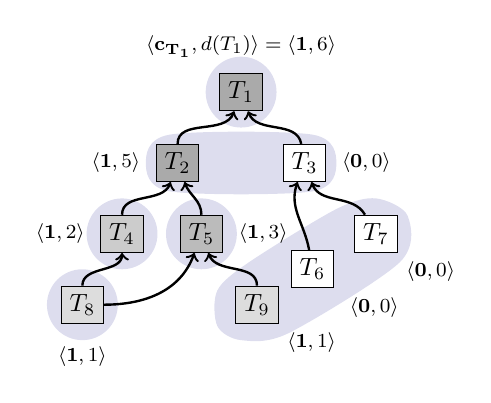
\begin{tikzpicture}[x=1.12cm, scale=0.9, every node/.append style={transform shape}]
    \begin{scope}[all/.style={draw, minimum height=0.5cm, minimum width=0.5cm},line width=0.08ex]
        \node[fill=lightgp, circle,minimum width=1cm] (pt1) at (0, 0) {};
        \node[fill=lightgp, circle,minimum width=1cm] (pt4) at (-1.5, -2) {};
        \node[fill=lightgp, circle,minimum width=1cm] (pt5) at (-0.5, -2) {};
        \node[fill=lightgp, circle,minimum width=1cm] (pt6) at (-2, -3) {};
        \fill[color=lightgp] plot[smooth cycle] coordinates { (1.2, -1) (0.9, -1.4) (-0.9, -1.4) (-1.2, -1) (-0.9, -0.6) (0.9, -0.6)} node (pt2) {};
        \fill[color=lightgp] plot[smooth cycle] coordinates {(2.1, -1.75) (2, -2.4) (0.6, -3.4) (0, -3.5) (-0.3, -3.3)(-0.3, -2.8) (0.1, -2.4) (1.2, -1.65) (1.7, -1.5) } node (pt3) {};
        \node[all, draw,fill=darkgray] (b0) at (0, 0) {$T_1$};
        \node[all, draw,fill=darkgray] (b1) at (-0.8, -1) {$T_2$};
        \node[all, draw,fill=white] (b2) at (0.8, -1) {$T_3$};
        \node[all, draw,fill=medgray] (b3) at (-1.5, -2) {$T_4$};
        \node[all, draw,fill=medgray2] (b4) at (-0.5, -2) {$T_5$};
        \node[all, draw,fill=white] (b5) at (0.9, -2.5) {$T_6$};
        \node[all, draw,fill=white] (b6) at (1.7, -2) {$T_7$};
        \node[all, draw,fill=lightgray] (b7) at (-2, -3) {$T_8$};
        \node[all, draw,fill=lightgray] (b8) at (0.2, -3) {$T_9$};
        \begin{scope}[line width=0.2ex]
        \path[->] (b1) edge[out=90, in=-110] node[sloped,above] {} (b0) ;
        \path[->] (b2) edge[out=100, in=-70] node[sloped,above] {} (b0) ;
        \path[->] (b3) edge[out=90, in=-110] node[sloped,above] {} (b1) ;
        \path[->] (b4) edge[out=90, in=-70] node[sloped,above] {} (b1) ;
        \path[->] (b5) edge[out=100, in=-110] node[sloped,above] {} (b2) ;
        \path[->] (b6) edge[out=120, in=-70] node[sloped,above] {} (b2) ;
        \path[->] (b7) edge[out=90, in=-90] node[sloped,above] {} (b3) ;
        \path[->] (b7) edge[out=0, in=-110] node[sloped,above] {} (b4) ;
        \path[->] (b8) edge[out=90, in=-70] node[sloped,above] {} (b4) ;
        \end{scope}
        %\node[] (p1) at (3, 0.5) {\footnotesize$\mathcal{P}_{T_1}$} ;
        %\node[] (p2) at (3, 0) {\footnotesize$\mathcal{P}_{T_2} = \mathcal{P}_{T_3}$};
        %\node[] (p3) at (3, -0.5) {\footnotesize$\mathcal{P}_{T_9} = \mathcal{P}_{T_6} = \mathcal{P}_{T_7}$};
        %\begin{scope}[color=darkgray,dashed,line width=0.2ex]
        %\path[->] (p1) edge[out=180, in=0] node[sloped,above] {} (pt1) ;
        %\path[->] (p2) edge[out=180, in=60] node[sloped,above] {} (pt2) ;
        %\path[->] (p3) edge[out=-90, in=30] node[sloped,above] {} (pt3) ;
        %\end{scope}

        \node[anchor=south, yshift=0.1cm] at (b0.north) {\footnotesize$\langle \mathbf{c_{T_1}}, d(T_1) \rangle = \langle\mathbf{1}, 6\rangle$};
        \node[anchor=east,xshift=-0.1cm] at (b1.west) {\footnotesize$\langle \mathbf{1}, 5 \rangle$};
        \node[anchor=west,xshift=0.1cm] at (b2.east) {\footnotesize$\langle \mathbf{0}, 0 \rangle$};
        \node[anchor=east,xshift=-0.1cm] at (b3.west) {\footnotesize$\langle \mathbf{1}, 2 \rangle$};
        \node[anchor=west,xshift=0.1cm] at (b4.east) {\footnotesize$\langle \mathbf{1}, 3 \rangle$};
        \node[anchor=north west,xshift=0.1cm] at (b5.south east) {\footnotesize$\langle \mathbf{0}, 0 \rangle$};
        \node[anchor=north west] at (b6.south east) {\footnotesize$\langle \mathbf{0}, 0 \rangle$};
        \node[anchor=north west] at (b8.south east) {\footnotesize$\langle \mathbf{1}, 1 \rangle$};
        \node[anchor=north,yshift=-0.2cm] at (b7.south) {\footnotesize$\langle \mathbf{1}, 1 \rangle$};
        
    \end{scope}
\end{tikzpicture}
}{\definecolor{lightgray}{HTML}{dddddd}
\definecolor{medgray}{HTML}{cccccc}
\definecolor{medgray2}{HTML}{bbbbbb}
\definecolor{darkgray}{HTML}{aaaaaa}
\definecolor{lightgp}{HTML}{ddddee}
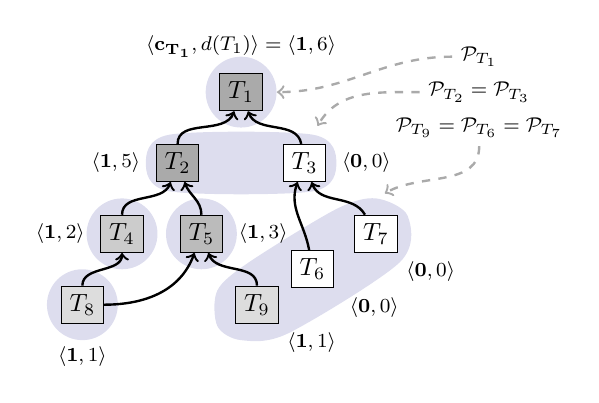
\begin{tikzpicture}[x=1.12cm, scale=0.9, every node/.append style={transform shape}]
    \begin{scope}[all/.style={draw, minimum height=0.5cm, minimum width=0.5cm},line width=0.08ex]
        \node[fill=lightgp, circle,minimum width=1cm] (pt1) at (0, 0) {};
        \node[fill=lightgp, circle,minimum width=1cm] (pt4) at (-1.5, -2) {};
        \node[fill=lightgp, circle,minimum width=1cm] (pt5) at (-0.5, -2) {};
        \node[fill=lightgp, circle,minimum width=1cm] (pt6) at (-2, -3) {};
        \fill[color=lightgp] plot[smooth cycle] coordinates { (1.2, -1) (0.9, -1.4) (-0.9, -1.4) (-1.2, -1) (-0.9, -0.6) (0.9, -0.6)} node (pt2) {};
        \fill[color=lightgp] plot[smooth cycle] coordinates {(2.1, -1.75) (2, -2.4) (0.6, -3.4) (0, -3.5) (-0.3, -3.3)(-0.3, -2.8) (0.1, -2.4) (1.2, -1.65) (1.7, -1.5) } node (pt3) {};
        \node[all, draw,fill=darkgray] (b0) at (0, 0) {$T_1$};
        \node[all, draw,fill=darkgray] (b1) at (-0.8, -1) {$T_2$};
        \node[all, draw,fill=white] (b2) at (0.8, -1) {$T_3$};
        \node[all, draw,fill=medgray] (b3) at (-1.5, -2) {$T_4$};
        \node[all, draw,fill=medgray2] (b4) at (-0.5, -2) {$T_5$};
        \node[all, draw,fill=white] (b5) at (0.9, -2.5) {$T_6$};
        \node[all, draw,fill=white] (b6) at (1.7, -2) {$T_7$};
        \node[all, draw,fill=lightgray] (b7) at (-2, -3) {$T_8$};
        \node[all, draw,fill=lightgray] (b8) at (0.2, -3) {$T_9$};
        \begin{scope}[line width=0.2ex]
        \path[->] (b1) edge[out=90, in=-110] node[sloped,above] {} (b0) ;
        \path[->] (b2) edge[out=100, in=-70] node[sloped,above] {} (b0) ;
        \path[->] (b3) edge[out=90, in=-110] node[sloped,above] {} (b1) ;
        \path[->] (b4) edge[out=90, in=-70] node[sloped,above] {} (b1) ;
        \path[->] (b5) edge[out=100, in=-110] node[sloped,above] {} (b2) ;
        \path[->] (b6) edge[out=120, in=-70] node[sloped,above] {} (b2) ;
        \path[->] (b7) edge[out=90, in=-90] node[sloped,above] {} (b3) ;
        \path[->] (b7) edge[out=0, in=-110] node[sloped,above] {} (b4) ;
        \path[->] (b8) edge[out=90, in=-70] node[sloped,above] {} (b4) ;
        \end{scope}
        \node[] (p1) at (3, 0.5) {\footnotesize$\mathcal{P}_{T_1}$} ;
        \node[] (p2) at (3, 0) {\footnotesize$\mathcal{P}_{T_2} = \mathcal{P}_{T_3}$};
        \node[] (p3) at (3, -0.5) {\footnotesize$\mathcal{P}_{T_9} = \mathcal{P}_{T_6} = \mathcal{P}_{T_7}$};
        \begin{scope}[color=darkgray,dashed,line width=0.2ex]
        \path[->] (p1) edge[out=180, in=0] node[sloped,above] {} (pt1) ;
        \path[->] (p2) edge[out=180, in=60] node[sloped,above] {} (pt2) ;
        \path[->] (p3) edge[out=-90, in=30] node[sloped,above] {} (pt3) ;
        \end{scope}

        \node[anchor=south, yshift=0.1cm] at (b0.north) {\footnotesize$\langle \mathbf{c_{T_1}}, d(T_1) \rangle = \langle\mathbf{1}, 6\rangle$};
        \node[anchor=east,xshift=-0.1cm] at (b1.west) {\footnotesize$\langle \mathbf{1}, 5 \rangle$};
        \node[anchor=west,xshift=0.1cm] at (b2.east) {\footnotesize$\langle \mathbf{0}, 0 \rangle$};
        \node[anchor=east,xshift=-0.1cm] at (b3.west) {\footnotesize$\langle \mathbf{1}, 2 \rangle$};
        \node[anchor=west,xshift=0.1cm] at (b4.east) {\footnotesize$\langle \mathbf{1}, 3 \rangle$};
        \node[anchor=north west,xshift=0.1cm] at (b5.south east) {\footnotesize$\langle \mathbf{0}, 0 \rangle$};
        \node[anchor=north west] at (b6.south east) {\footnotesize$\langle \mathbf{0}, 0 \rangle$};
        \node[anchor=north west] at (b8.south east) {\footnotesize$\langle \mathbf{1}, 1 \rangle$};
        \node[anchor=north,yshift=-0.2cm] at (b7.south) {\footnotesize$\langle \mathbf{1}, 1 \rangle$};
        
    \end{scope}
\end{tikzpicture}
}
    \definecolor{lightgray}{HTML}{dddddd}
\definecolor{medgray}{HTML}{cccccc}
\definecolor{medgray2}{HTML}{bbbbbb}
\definecolor{darkgray}{HTML}{aaaaaa}
\definecolor{lightgp}{HTML}{ddddee}
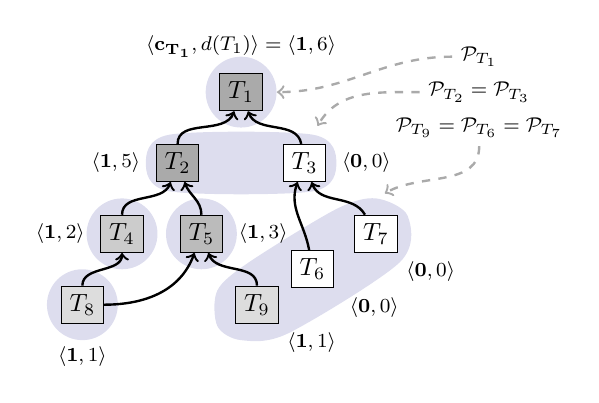
\begin{tikzpicture}[x=1.12cm, scale=0.9, every node/.append style={transform shape}]
    \begin{scope}[all/.style={draw, minimum height=0.5cm, minimum width=0.5cm},line width=0.08ex]
        \node[fill=lightgp, circle,minimum width=1cm] (pt1) at (0, 0) {};
        \node[fill=lightgp, circle,minimum width=1cm] (pt4) at (-1.5, -2) {};
        \node[fill=lightgp, circle,minimum width=1cm] (pt5) at (-0.5, -2) {};
        \node[fill=lightgp, circle,minimum width=1cm] (pt6) at (-2, -3) {};
        \fill[color=lightgp] plot[smooth cycle] coordinates { (1.2, -1) (0.9, -1.4) (-0.9, -1.4) (-1.2, -1) (-0.9, -0.6) (0.9, -0.6)} node (pt2) {};
        \fill[color=lightgp] plot[smooth cycle] coordinates {(2.1, -1.75) (2, -2.4) (0.6, -3.4) (0, -3.5) (-0.3, -3.3)(-0.3, -2.8) (0.1, -2.4) (1.2, -1.65) (1.7, -1.5) } node (pt3) {};
        \node[all, draw,fill=darkgray] (b0) at (0, 0) {$T_1$};
        \node[all, draw,fill=darkgray] (b1) at (-0.8, -1) {$T_2$};
        \node[all, draw,fill=white] (b2) at (0.8, -1) {$T_3$};
        \node[all, draw,fill=medgray] (b3) at (-1.5, -2) {$T_4$};
        \node[all, draw,fill=medgray2] (b4) at (-0.5, -2) {$T_5$};
        \node[all, draw,fill=white] (b5) at (0.9, -2.5) {$T_6$};
        \node[all, draw,fill=white] (b6) at (1.7, -2) {$T_7$};
        \node[all, draw,fill=lightgray] (b7) at (-2, -3) {$T_8$};
        \node[all, draw,fill=lightgray] (b8) at (0.2, -3) {$T_9$};
        \begin{scope}[line width=0.2ex]
        \path[->] (b1) edge[out=90, in=-110] node[sloped,above] {} (b0) ;
        \path[->] (b2) edge[out=100, in=-70] node[sloped,above] {} (b0) ;
        \path[->] (b3) edge[out=90, in=-110] node[sloped,above] {} (b1) ;
        \path[->] (b4) edge[out=90, in=-70] node[sloped,above] {} (b1) ;
        \path[->] (b5) edge[out=100, in=-110] node[sloped,above] {} (b2) ;
        \path[->] (b6) edge[out=120, in=-70] node[sloped,above] {} (b2) ;
        \path[->] (b7) edge[out=90, in=-90] node[sloped,above] {} (b3) ;
        \path[->] (b7) edge[out=0, in=-110] node[sloped,above] {} (b4) ;
        \path[->] (b8) edge[out=90, in=-70] node[sloped,above] {} (b4) ;
        \end{scope}
        \node[] (p1) at (3, 0.5) {\footnotesize$\mathcal{P}_{T_1}$} ;
        \node[] (p2) at (3, 0) {\footnotesize$\mathcal{P}_{T_2} = \mathcal{P}_{T_3}$};
        \node[] (p3) at (3, -0.5) {\footnotesize$\mathcal{P}_{T_9} = \mathcal{P}_{T_6} = \mathcal{P}_{T_7}$};
        \begin{scope}[color=darkgray,dashed,line width=0.2ex]
        \path[->] (p1) edge[out=180, in=0] node[sloped,above] {} (pt1) ;
        \path[->] (p2) edge[out=180, in=60] node[sloped,above] {} (pt2) ;
        \path[->] (p3) edge[out=-90, in=30] node[sloped,above] {} (pt3) ;
        \end{scope}

        \node[anchor=south, yshift=0.1cm] at (b0.north) {\footnotesize$\langle \mathbf{c_{T_1}}, d(T_1) \rangle = \langle\mathbf{1}, 6\rangle$};
        \node[anchor=east,xshift=-0.1cm] at (b1.west) {\footnotesize$\langle \mathbf{1}, 5 \rangle$};
        \node[anchor=west,xshift=0.1cm] at (b2.east) {\footnotesize$\langle \mathbf{0}, 0 \rangle$};
        \node[anchor=east,xshift=-0.1cm] at (b3.west) {\footnotesize$\langle \mathbf{1}, 2 \rangle$};
        \node[anchor=west,xshift=0.1cm] at (b4.east) {\footnotesize$\langle \mathbf{1}, 3 \rangle$};
        \node[anchor=north west,xshift=0.1cm] at (b5.south east) {\footnotesize$\langle \mathbf{0}, 0 \rangle$};
        \node[anchor=north west] at (b6.south east) {\footnotesize$\langle \mathbf{0}, 0 \rangle$};
        \node[anchor=north west] at (b8.south east) {\footnotesize$\langle \mathbf{1}, 1 \rangle$};
        \node[anchor=north,yshift=-0.2cm] at (b7.south) {\footnotesize$\langle \mathbf{1}, 1 \rangle$};
        
    \end{scope}
\end{tikzpicture}

%O     \captionof{figure}{Example of $\langle \textrm{chit}, \textrm{confidence}\rangle$ values.  Darker boxes indicate transactions with higher confidence values. At most one transaction in each shaded region will be accepted.}
    \captionof{figure}{Exemple de valeurs pour $\langle \textrm{chit}, \textrm{confidence}\rangle$. Les boîtes sombres indiquent des transactions dont l'indice de confiance est supérieur. Au plus une transaction dans chaque région ombrée sera acceptée.}
    \label{fig:dag-cd}
\end{center}
\end{figure}

%O Figure~\ref{fig:dag-cd} illustrates a sample DAG built by Avalanche.
La Figure~\ref{fig:dag-cd} illustre un exemple de DAG construit par Avalanche.
%O Similar to Snowball, sampling in Avalanche will create a positive feedback for the preference of a single transaction in its conflict set.
De même que pour Snowball, l'échantillonnage dans Avalanche créer une rétroaction positive pour la préférence d'une seule transaction dans sont ensemble de conflit.
%O For example, because $T_2$ has larger confidence than $T_3$, its descendants are more likely collect chits in the future compared to $T_3$.
Par exemple, comme $T_2$ a un indice de confiance supérieur à celui de $T_3$, ses descendants seront plus à même de récolter des \emph{chits} à l'avenir que $T_3$.

%O \tronly{Similar to Bitcoin, Avalanche leaves determining the acceptance point of a transaction to the application. An application supplies an \textsc{isAccepted} predicate that can take into account the value at risk in the transaction and the chances of a decision being reverted to determine when to decide.}{}
\tronly{Comme Bitcoin, Avalanche laisse à l'application le soin de déterminer le point d'acceptation d'une transaction. Une application fournit un prédicat \textsc{isAccepted} qui peut prendre en compte la valeur en jeu dans la transaction et les chances de réversion d'une décision pour déterminer le moment de cette décision.}{}

%O Committing a transaction can be performed through a \emph{safe early commitment}. For virtuous transactions, $T$ is accepted when it is the only transaction in its conflict set and has a confidence not less than threshold $\beta_1$.
L'engagement concernant une transaction peut être effectié par un \emph{engagement préalable sûr}. Pour les transactions vertueuses, $T$ est acceptée quand elle est la seule transaction dans son ensemble de conflit et que sa confiance n'est pas inférieure à un seuil $\beta_1$.
%O As in Snowball, $T$ can also be accepted after a $\beta_2$ number of consecutive successful queries.
Comme dans Snowball, $T$ peut aussi être acceptée après un nombre de requêtes réussies consécutives $\beta_2$.
%O If a virtuous transaction fails to get accepted due to a problem
%O with parents, it could be accepted if reissued with different parents.
Si une transaction vertueuse échoue à être acceptée en raison d'un problème avec ses parents elle peut être acceptée si elle est réémise avec des parents différents.
%O Figure~\ref{fig:gossipchain-ongen} shows how Avalanche entangles transactions. Because transactions that consume and generate the same UTXO do not conflict with each other, any transaction can be reissued with different parents.
La Figure~\ref{fig:gossipchain-ongen} montre comment Avalanche lie les transactions entre elles. Puisque les transactions qui consomment et génèrent la même UTXO n'entrent pas en conflit entre elles, toute transaction peut être réémise avec des parents différents.

\tronly{
%O Figure~\ref{fig:gossipchain-main} illustrates the protocol main loop
%O executed by each node.
La igure~\ref{fig:gossipchain-main} illustre la boucle principale du protocole exécutée par chaque nœud.
%O In each iteration, the node attempts to select a transaction $T$ that has not
%O yet been queried.  If no such
%O transaction exists, the loop will stall until a new transaction is
%O added to $\mathcal{T}$.
À chaque itération, le nœud tente de sélectionner une transaction $T$ qui n'a pas encore été interrogée. 
S'il n'existe pas de telle transaction, la boucle se met en pause jusqu'à ce qu'une nouvelle transaction soit ajoutée à $\mathcal{T}$.
%O It then selects $k$ peers and queries those peers.
Il sélectionne ensuite $k$ pairs et les interroge.
%O If more than $\alpha$ of those peers return a positive response, the chit value is set to~1.
Si plus que $\alpha$ de ces pairs reviennent à une réponse positive, la valeur de \emph{chit} est mise à~1.
%O After that, it updates the preferred transaction of each conflict set
%O of the transactions in its ancestry.
Après cela, il met à jour la transaction qu'il préfère de chaque ensemble de conflits des transactions dans son ascendance.
%O Next, $T$ is added to the set $\mathcal{Q}$
%O so it will never be queried again by the node.
Ensuite, $T$ est ajoutée à l'ensemble $\mathcal{Q}$ afin de ne plus jamais être interrogée par le nœud.
%O The code that selects additional peers if some of the $k$ peers are
%O unresponsive is omitted for simplicity.
Le code qui sélectionne des pairs supplémentaires sur certains des $k$ pairs ne répondent pas est omis dans un but de simplicité.

%O Figure~\ref{fig:gossipchain-onquery} shows what happens when a node
%O receives a query for transaction $T$ from peer $j$.
La Figure~\ref{fig:gossipchain-onquery} montre ce qui se produit quand un nœud reçoir une requête pour la transaction $T$ du pair $j$.
%O First it adds $T$ to $\mathcal{T}$, unless it already has it.
Il ajoute d'abord $T$ à $\mathcal{T}$, à moins qu'il ne l'ait déjà.
%O Then it determines if $T$ is currently strongly preferred.
Il détermine ensuite si $T$ est actuellement fortement préféré.
%O If so, the node returns a positive response to peer $j$.
Dans ce cas, le nœud renvoie une réponse positive au pair $j$.
%O Otherwise, it returns a negative response.
Sinon, il renvoie une réponse négative.
%O Notice that in the pseudocode, we assume when a node knows $T$, it also
%O recursively knows the entire ancestry of $T$. This can be achieved by
%O postponing the delivery of $T$ until its entire ancestry is recursively
%O fetched.
On remarque que, dans le pseudocode, nous assumons que quand un nœud connaît $T$, il connaît aussi récursivement toute son ascendance.
Cela peut être réalisé en retardant la délivrance de $T$ jusqu'à ce que l'intégralité de son ascendance soit récursivement récupérée.
%O In practice, an additional gossip process that disseminates
%O transactions is used in parallel, but is not shown in pseudocode for simplicity.
En pratique, un processus \emph{gossip} supplémentaire qui dissémine des transaction est utilisé en parallèle, mais n'est pas montré dans le pseudocode dans un but de simplicité.
}{}
